\section{Design}\label{sec:design}
In this chapter, I am going to describe the design steps realized during the implementation of the demonstrator. Section \ref{subsec:exampleforimplementation} describes all the examples that I have conceptualized before choosing the final one for the implementation. This is then followed by the description of the steps taken for selecting the bx-tool in Section \ref{subsec:bxtoolselection}. Afterwards, Section \ref{subsec:architecturedesign} deals with the decisions taken for finalizing the application's architecture design. Then, Section \ref{subsec:design_layers} describes the application's framework in detail along with its components. Afterwards, Section \ref{subsec:designchallenges} describes the challenges that I faced while designing the entire framework and its components. At last, Section \ref{subsec:choicesthreats} describes some of the choices that I made during the design phase and its associated threats. 

\subsection{Choosing an Example}\label{subsec:exampleforimplementation}
To solve the problems as described in Section \ref{subsec:probstmt}, the main idea is to design and implement an interactive bx tool demonstrator based on an intuitive example.

\subsubsection{Construction}\label{subsubsec:exampleconstruction}
I have constructed a few examples for implementation as follows:

\paragraph{Task Management} This prototype can be used for allocating tasks in a team. It contains two views e.g., supervisor's view and employee's view. A supervisor can allocate tasks to their subordinates. An employee can view the tasks assigned to him. Then the task will go through a life cycle as the work progresses, i.e., Assigned, In Progress, Testing, Done. Supervisor's view shows aggregate information from multiple projects and multiple employees, but does not contain detailed information, e.g., tasks have fewer states than for assigned employees. Bx rules control how updates are handled and states are reflected in the different views of the project, e.g., the employee's view will be updated for each state change, whereas the supervisor's view is only updated when a task is completed and not for intermediate changes.

\paragraph{Quiz} This prototype can be used for an online quiz game. It contains two views e.g., administrator's view and participant's view.
There will be a large set of questions related to different areas, e.g, history, geography, politics, sports, etc. The administrator can select the areas from which the questions will be shown to the participant and initiate the game. The participant can override the selection of the areas and start the quiz. Randomly questions will be shown to the participant from the selected areas with 4 options. The administrator's view contains less information than the participant's view, e.g., only the result of each question will be shown to the administrator, whereas participant can see questions along with its options. As soon as the participant chooses the answer to any question, bx rules control how updates are handled and states are reflected in the different views of the project.

\paragraph{Playing with Shapes} It contains two views e.g., low-level view (depicts \ac{UI} for low-level language, i.e., UI with less functionality) and high-level view (depicts UI for high-level language, i.e., UI with more functionality). User will draw a geometric shape, i.e., triangle / square / rectangle / circle with some notations similar to the shape on the low-level view and if the notations are correct, the high-level view tries to recognize the shape and draws it with default parameters and vice-versa. Basically the transformation will happen between a low-level language and a high-level language and bx rules control how updates are handled and states are reflected in the different views of the project. In high-level view, more functionalities will be present, i.e., moving one shape from one place to another, creating a clone of an existing shape, etc. which is not possible in low-level view.

\paragraph{Arranging a Kitchen}
It contains two views e.g., low-level view (depicts a grid structure containing blocks) and high-level view (empty space which depicts UI for kitchen). High-level view has more functionalities such as creating/ deleting/ moving an kitchen item, etc. out of which only a few will be available in low-level view. User will create/ delete/ move a kitchen item, i.e., sink / table on the high-level view and if changes done on the high-level view are according to the rules defined in the bx tool then items will be reflected on the low-level view with same colored blocks and vice-versa. Basically the transformation will happen between a low-level language and a high-level language and bx rules control how updates are handled and states are reflected in the different views of the project.

\paragraph{Person and Family}
The concept of this example is taken from the example \emph{FamilyToPersons} located in the bx examples repository~\cite{bx-examples}. It contains two views e.g., Family view and Person view. In Family view, it contains many families and each family consist of members. Whereas, Person view contains persons (the members of each family). We assume that the surnames are unique and allow us to differentiate between different families. Addition of a new person to the Person view will be reflected on the family view and vice-versa. Also, due to the uniqueness of the surnames, person created will be automatically assigned to the related family. Bx rules control how updates are handled and states are reflected in the different views.

\subsubsection{Selection}\label{subsubsec:exampleselection}
Selecting an example for the demonstrator was not random, rather I have taken many factors into considerations before choosing the final one. It was a very important decision, as selection of the example and its implemenation will directly effect the research question \textit{RQ 4} specified in Section \ref{subsec:probstmt} and requirements \textit{NR 2}, \textit{NR 3} described in Section \ref{subsec:nonfunctionalreq}.

Hence by taking into account all these factors, I have constructed a few evaluation criterias (referred to as \textbf{EC}) for the selection process of the most suitable example as listed below:
\begin{description}
	\item [EC 1:] User should be familiar with the example.
	\item [EC 2:] Example should be simple without the involvement of any technical details.
	\item [EC 3:] Interactivity should not create a overhead for the user but rather be intuitive.
	\item [EC 4:] User should be able to relate to the learning concepts through the example.
\end{description}

Table~\ref{tab:comparison_examples} shows the comparison of the examples based on the evaluation criterias. "\checkmark" denotes the fulfillment of the evaluation criteria whereas, "\ding{55}" denotes the non-fulfillment of the evaluation criteria. This comparison table clearly shows that \textit{Arranging a Kitchen} is the most suitable example. It fulfills all the evaluation criterias because any user can relate to the example very well as everybody is familiar with a kitchen and its environment, example is very simple and no technical details are involved, interactivity and rules won't be a overhead for the user as the environment is a part of day to day life and hence user will be able to relate to the learning concepts through the example. So, I have finally chosen this example for the demonstrator and also as part of my research.

\begin{table}
	\centering
	\begin{tabular}{|lcccc|}
		\hline
		\textbf{} & \multicolumn{4}{c|}{\textbf{Evaluation Criterias}} \\
		\textbf{Examples} & \textbf{EC1} & \textbf{EC2} & \textbf{EC3} & \textbf{EC4} \\
		\hline
		\hline
		Task Management & \ding{55} & \ding{55} & \checkmark & \checkmark \\ 
		\hline
		Quiz & \checkmark & \ding{55} & \checkmark & \checkmark \\
		\hline
		Playing with Shapes & \ding{55} & \ding{55} & \checkmark & \checkmark \\
		\hline
		Person and Family & \checkmark & \checkmark & \ding{55} & \checkmark \\
		\hline
		Arranging a Kitchen & \checkmark &  \checkmark & \checkmark & \checkmark \\
		\hline
	\end{tabular}
	\caption{Comparison of examples based on evaluation criterias}
	\label{tab:comparison_examples}
\end{table}

\subsection{BX Tool Selection}\label{subsec:bxtoolselection}
Next step in the design process was selection of a bx tool which takes care of the bx part of the demonstrator and upon which the entire framework of the demonstrator will be constructed. My gathered information during the case study phase led the foundation for the selection process.

\subsubsection{Case Study}\label{subsubsec:bxtoolcasestudy}
I further investigated on the existing bx tools from the point of view of practical application and usage of these tools in terms of building softwares. Even after a significant amount of work has been done by developers community and bx community, the main problems were revolving around the conceptual, practical challenges associated with using bx, and tool/technology in building software systems and absence of benchmarks for comparison of complete bx solutions~\cite{bx-theoryandappl}.

To focus particularly on these issues, bx-community had conducted a series of technical workshops at relevant conferences and organised week-long intensive research seminars~\cite{bx-theoryandappl}. Some of the main outcome of these seminars are listed below:
\begin{itemize}
	\item {focus on the need of benchmarks and further categorizing them into functional and non-functional ones.}
	\item {software tool support for bx was shown in terms of demos which includes tool like eMoflon, Echo etc.}
\end{itemize}

\subsubsection{Selection}\label{subsubsec:bxtoolselection}
Again, it was a very important decision, as selection of the bx tool and the implemenation on the top of it will directly effect the research questions \textit{RQ 1}, \textit{RQ 2}  specified in Section \ref{subsec:probstmt}.

The outcome of the seminars as discussed in previous section \ref{subsubsec:bxtooltheory} led me to concentrate and analyze the bx tools like eMoflon, Echo, BIGUL. Also, I came across the benchmark \cite{benchmarx} \cite{benchmarx-reload}, the first non-trivial benchmark where Anjorin et al. has provided a practical framework to compare and evaluate three bx tools. After analyzing these tools, benchmarks and taking into consideration the reserach questions and requiements, I have finally chosen \textit{eMoflon} as the bx tool to handle the bx part of the demonstrator. Following were the driving factors for the selection of the bx tool:
\begin{itemize}
	\item {sample implementation with framework to implement the eMoflon tool was already available.}
	\item {my supervisor/prof. is a core member of the eMoflon developer team which gave me added advantage of knowing the tool inside out. This extra knowledge actually helped me in solving the implemenation issues/challenges related to the tool.}
	\item {eMoflon is Java based and was thus easier for me to integrate and work with, compared to BiGUL (Haskell-based).}
\end{itemize}

\subsubsection{Benchmarx}\label{subsubsec:benchmarx}
A bx benchmark (referred to as \textbf{Benchmarx} from now on) is a bx example that has a precise and executable definition of a binary consistency relation on source and target artefacts; an explicit definition of, or a generator for, input artefact elements; a set of precisely defined update scenarios for certain input artefact elements; and a set of executable metric definitions \cite{bx-theoryandappl}.
\newline\newline Anjorin et al. \cite{benchmarx-reload} tried to solve the main problem with benchmarking bx tools by creating a common design space, in which different bx tools architecture can be accomodated irrespective of the fact that they can have different input data. 

\paragraph{Design Space} 

\subsection{Architecture Design}\label{subsec:architecturedesign}
Last step in the design process was application architecture design which is the most important part of my thesis and also the starting phase of the implementation of the prototype.

I decided to build a web appliaction to address the requirements \textit{FREQ1}, \textit{NREQ1} and \textit{NREQ2} described in Section \ref{subsec:functionalreq} and \ref{subsec:nonfunctionalreq}.
\newline\newline Web application development has evolved drastically from single page design to very complex layering structures since the beginning of World Wide Web. Many design patterns \cite{designpattern} \cite{designpattern-notes} consisting of different technologies and programming languages were proposed, adopted and implemented in different time to address the demands of customers and users on web. With the rapid changes occuring on World Wide Web, technologies are becoming obsolete and losing its demand day by day. Nowadays, the main focus is on improving the user interaction and allow the developers to build powerful web applications rapidly.
\newline\newline I have analyzed a few design patterns and commonly used architecture designs in todays world by working on a few Proof of Concepts (PoC). Main goal of my thesis is to design and implement a demonstrator based on a bx-tool as described in Section \ref{subsec:contribution} and prior to this stage, I have already selected \textit{eMoflon} as my bx-tool in Section \ref{subsec:bxtoolselection}. So, The main idea was to check the feasibility of the architecture and the data flow within its components on the top of the interface provided by the \textit{Benchmarx} (proposed by Anjorin et al. \cite{benchmarx-reload}) to access the bx-tool. While working on the PoCs, I came across a few problems such as, maintainability and reusability of code, dependencies of components etc. To avoid these problems and to address the requirement \textit{NREQ3} described in Section \ref{subsec:functionalreq}, I finally chose Model-View-Controller (referred as \textbf{MVC} from now on) architecture for my application framework. Following were the driving factors for the selection of the MVC architecture \cite{designpattern-notes} \cite{designpattern-headfirst} :
\begin{itemize}
	\item {it differentiates the layers of a project in Model, View and Controller for the re-usability and easy maintainance of code.}
	\item {it splits responsibilities into three main roles which allows the developers to work independently without interfering in each others work and for more efficient collaboration.}
	\item {due to the sepration of concern, same Model can have any no.of Views. Enhancements in Views and other support of new technologies for building the View can be implemented easily.}
	\item {a person who is working on View does not need to know about the underlying Model code base and its architecture.}
\end{itemize}

\begin{figure}
	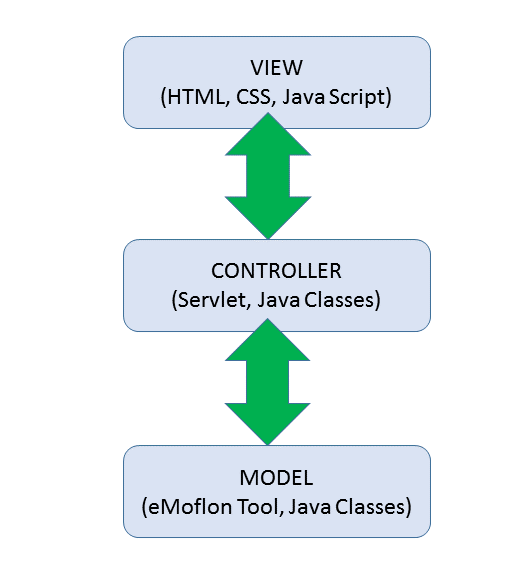
\includegraphics[width=1\textwidth]{figures/Highlevel_Arch}
	\caption{High Level Architecture Diagram}
	\label{fig:Architecture_Diagram}
\end{figure}

\subsection{Architecture Layers}\label{subsec:design_layers}
Figure~\ref{fig:Architecture_Diagram} shows a very high-level architecture diagram of my prototype. It consist of 3 components e.g., Model, View and Controller. View is responsible for all the graphical user interface management and consist of technologies like HTML, CSS, JavaScript and Jquery. Controller is responsible for event handling and basically consist of the technology Servlet. Model is responsible for all the tasks related to business logic, business rules, data, meta-models, state of meta-models etc. and consist of java classes.

\paragraph{Request-Response Cycle} 
Figure~\ref{fig:Detail_Architecture_Diagram} shows a detailed architecture diagram with a complete request-response cycle described below:
\begin{enumerate}
	\item {User interacts with the application on a browser and user actions are sent to the Controller as requests.}
	\item {After accepting the request, Controller decides on how to handle it and send it to the controller helper for further processing.}
	\item {After processing the request, controller helper send it to the Model.}
	\item {Model processes the request and generates the response, which is sent back to the controller through controller helper.}
	\item {After receiving the response, Controller prepares the data and send it to the View.}
	\item {View processes the data and finally the final response is generated and loaded on the browser.}
\end{enumerate}

\begin{sidewaysfigure}
	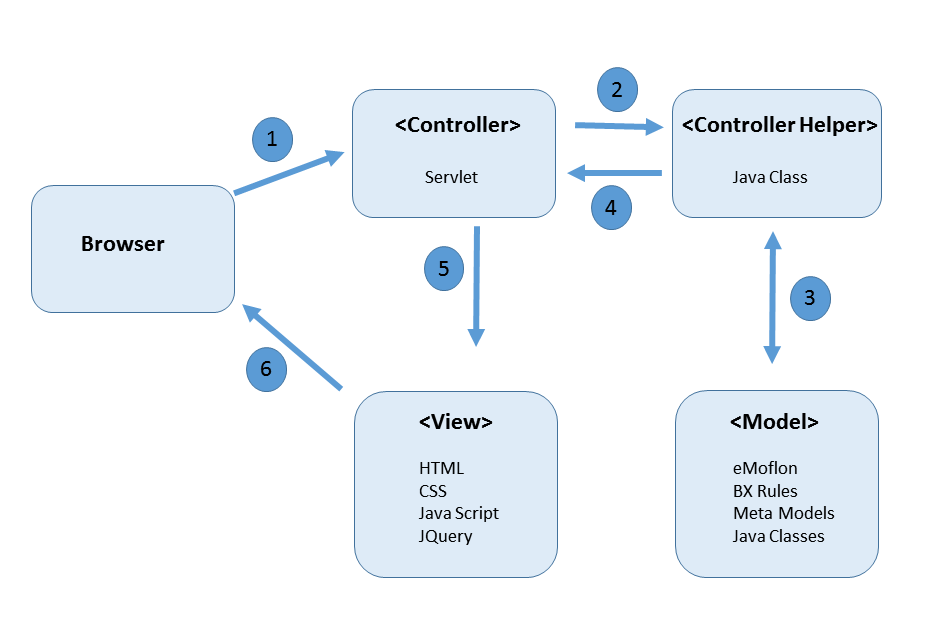
\includegraphics[width=1\textwidth]{figures/Detail_Arch}
	\caption{Detail Architecture Diagram}
	\label{fig:Detail_Architecture_Diagram}
\end{sidewaysfigure}

Below sub-sections describes the designing process of each component e.g., Model, View and Controller in detail.

\subsubsection{Model}\label{subsubsec:design_model}
Model is mainly responsible for encapsulating the access of data and handling the business logic of the application \cite{designpattern-headfirst} \cite{mvc-arch}. It ensures the data abstraction and provides methods to access it, due to which the complexity of writing the code on developers' part is highly reduced \cite{mdd-webwithmvc}.
\newline\newline In my case, Model is consist of java classes and the \textit{eMoflon} tool. The java classes consist of interfaces and its concrete implementation designed to access the bx-tool eMoflon on the top of the framework provided by the \textit{Benchmarx}. The tool contains all the meta-models, state of the meta-models and the associated transformation rules.

\paragraph{eMoflon specific Models}
For implementing the example \textit{Arranging a Kitchen} through \textit{eMoflon} tool, first task was to create related models inside the tool. The bx tool will keep these models, create and manage instances of these models by applying associted transformation rules as per the requirement. As the example has two different views, it requires two different model in the tool as well i.e., \texttt{KitchenLanguage} to represent high-level view and \texttt{GridLanguage} to represent low-level.

\begin{figure}
	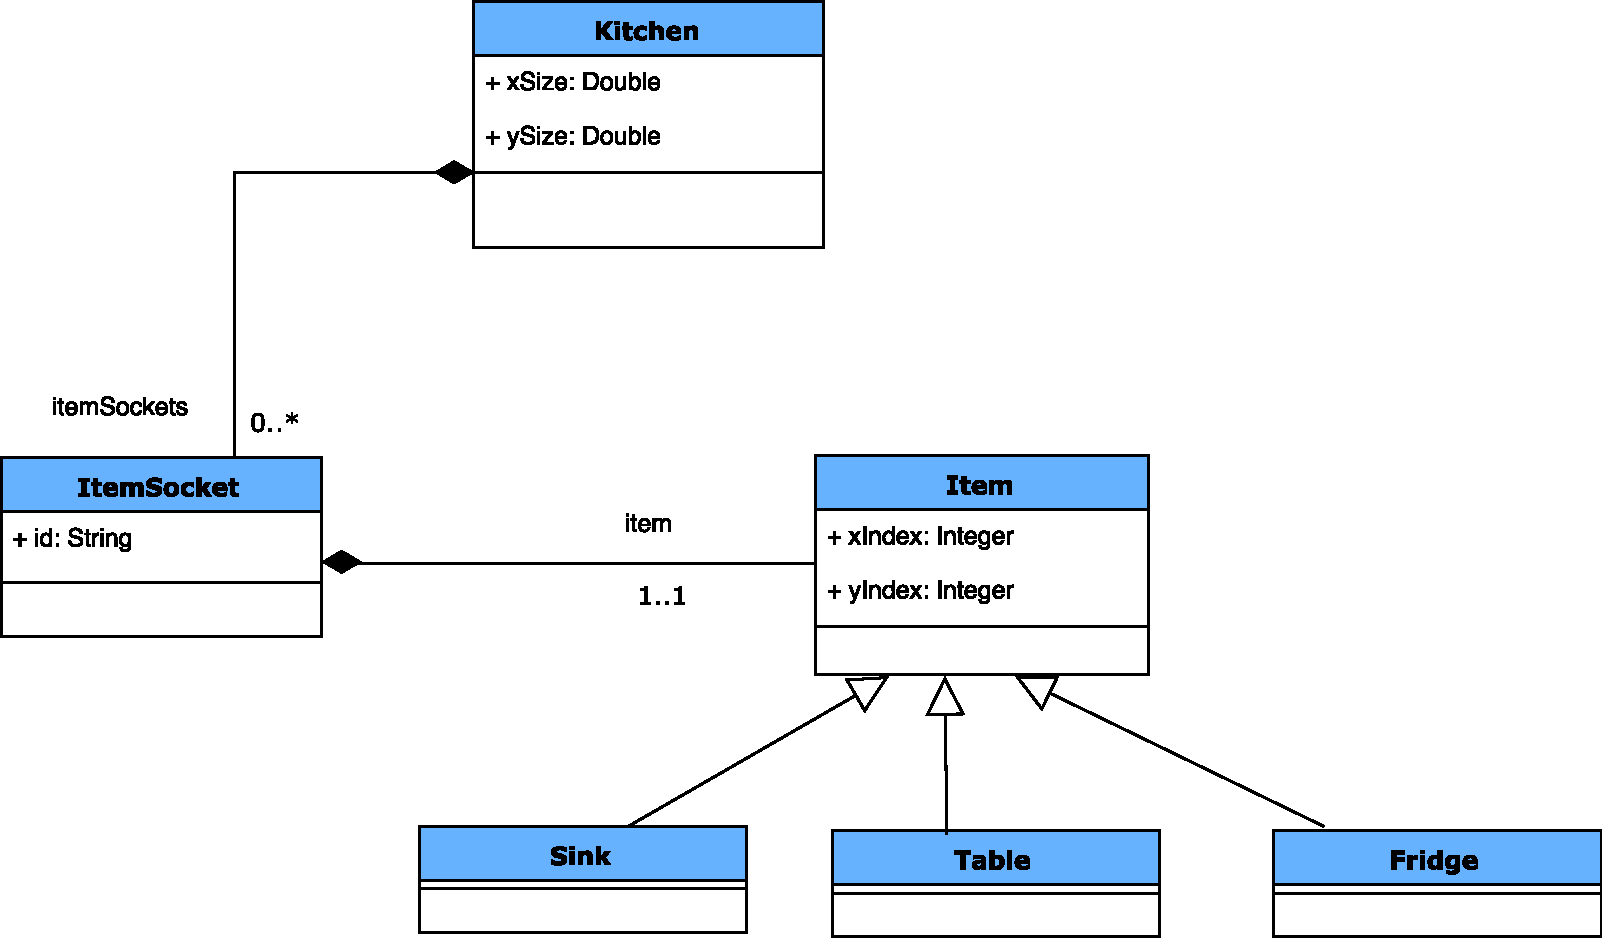
\includegraphics[width=1\textwidth]{figures/ClassDia_KitchenLanguage}
	\caption{KitchenLanguage Class Diagram}
	\label{fig:ClassDia_KitchenLanguage}
\end{figure}

Figure~\ref{fig:ClassDia_KitchenLanguage} describes the structure of the \texttt{KitchenLanguage} model in a class diagram from an object-oriented point of view. It contains three classes i.e., \texttt{Kitchen}, \texttt{ItemSocket}, and \texttt{Item}. \texttt{Kitchen} class has the attributes \textit{xSize} and \textit{ySize} to describe its size and contains zero or more itemsockets. \texttt{ItemSocket} class has the attribute \textit{id} and contains exactly one item. \texttt{Item} class has the attributes \textit{xIndex} and \textit{yIndex} to describe its position. \texttt{Sink}, \texttt{Table}, and \texttt{Fridge} are different types of items.

\begin{figure}
	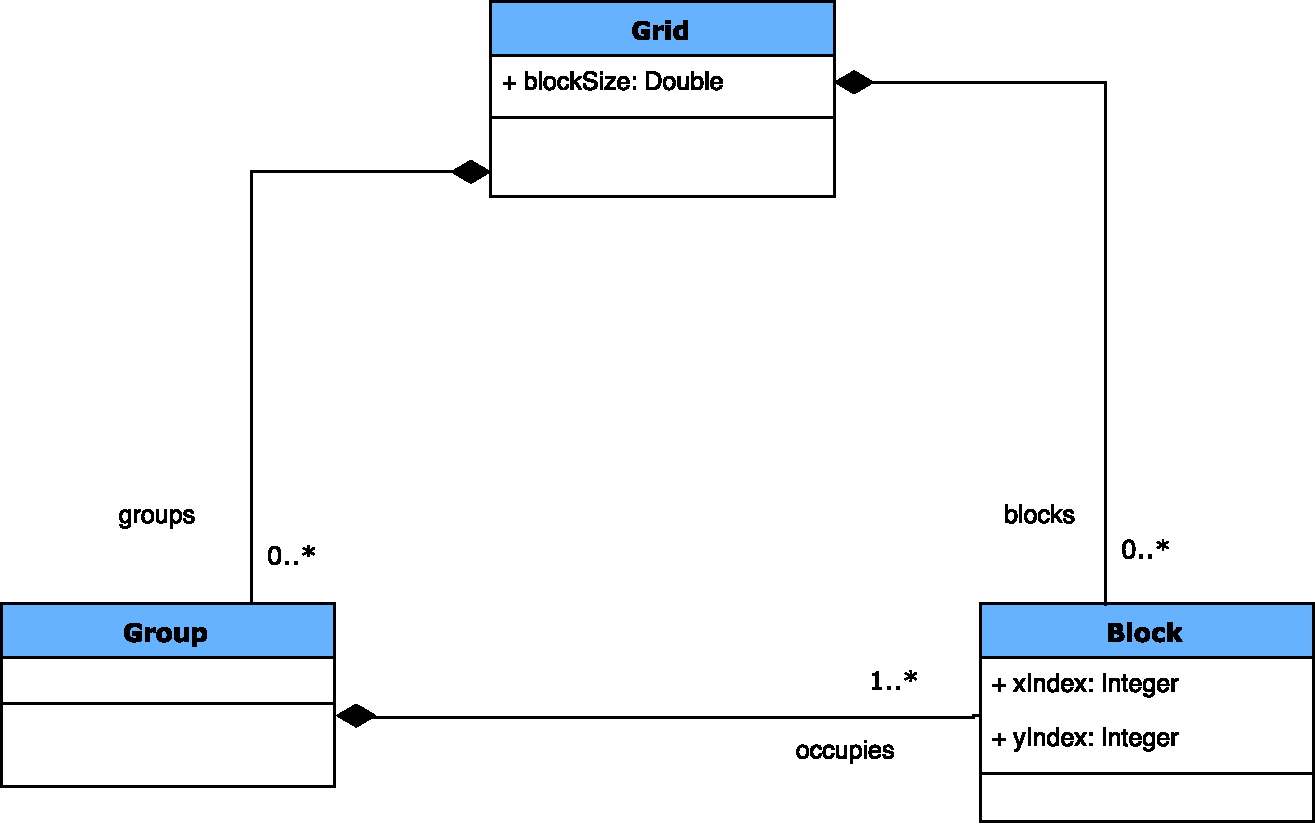
\includegraphics[width=1\textwidth]{figures/ClassDia_GridLanguage}
	\caption{GridLanguage Class Diagram }
	\label{fig:ClassDia_GridLanguage}
\end{figure}

Figure~\ref{fig:ClassDia_GridLanguage} describes the structure of the \texttt{GridLanguage} model in a class diagram from an object-oriented point of view. It contains three classes i.e., \texttt{Grid}, \texttt{Group}, and \texttt{Block}. \texttt{Grid} class has the attribute \textit{blockSize} to describe the size of each blocks contained inside it, contains zero or more itemsockets, and zero or more blocks. Each \texttt{Group} class occupies one or more blocks. \texttt{Block} class has the attributes \textit{xIndex} and \textit{yIndex} to describe its position and is being occupied by one group.

\begin{sidewaysfigure}
	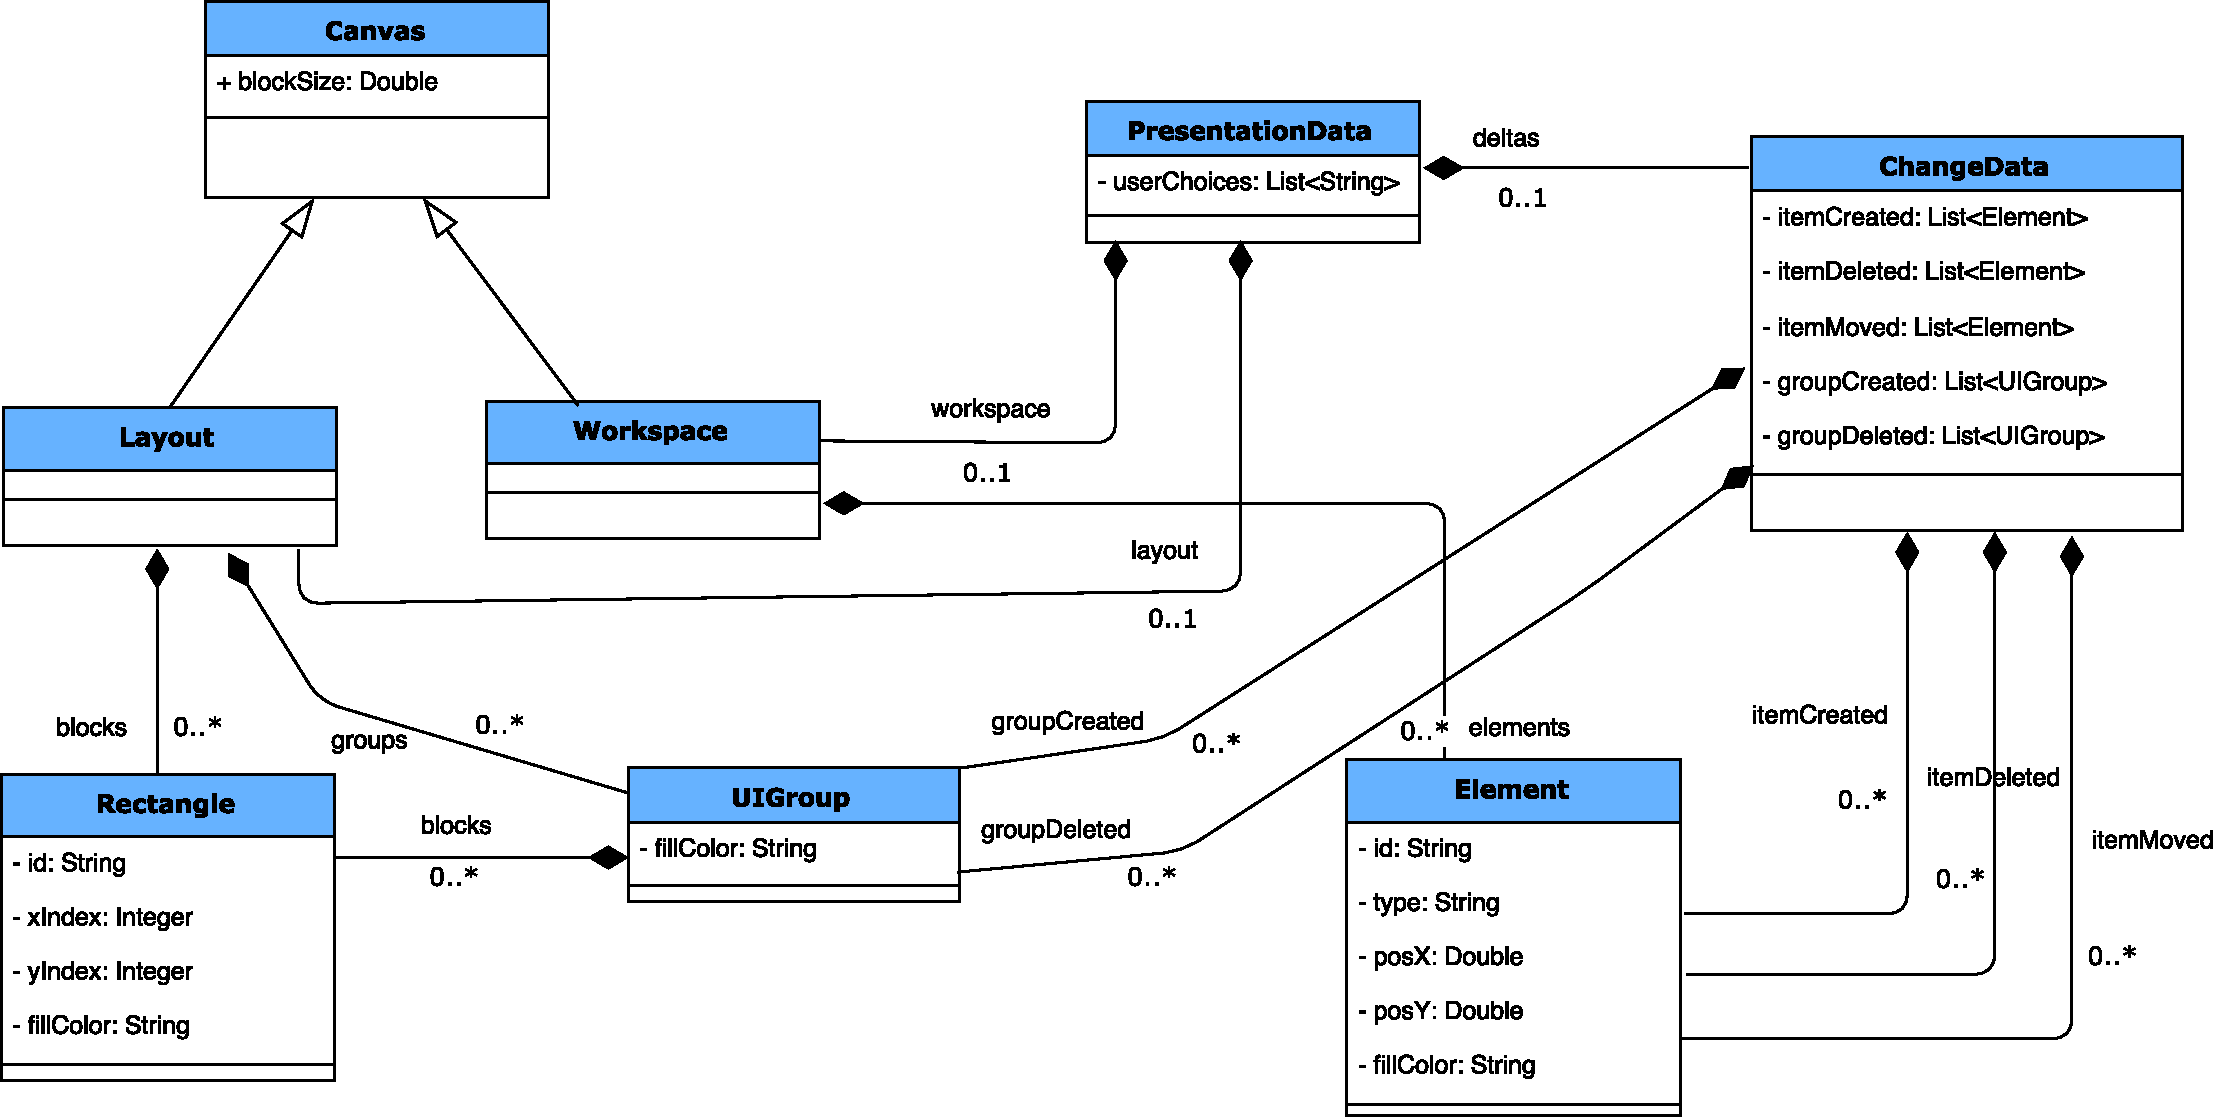
\includegraphics[width=1\textwidth]{figures/ClassDia_UI-Models}
	\caption{Structure and Relationship between UI Models}
	\label{fig:ClassDia_UI-Models}
\end{sidewaysfigure}

\paragraph{UI related Models}
Now, the second step in modeling was to create models for user interface to handle and visualize the bx tool specific models. Thus, UI models are necessary to deal with the user actions and act a connecting bridge between the user actions and the bx tool specific models. While user interacts with the demonstartor, actions i.e., changes performed by the user in the UI will be captured in the form of the UI models and will be sent to the controller helper. Conversion between the UI models and bx tool specific models happens inside the controller helper before sending the request to the bx tool 
and after receiving the response from the bx tool. View always receives the response in the form of UI models and visualize them.

Figure~\ref{fig:ClassDia_UI-Models} describes the structure and relationship between the models related to user interface in a class diagram. UI models consist of classes like \texttt{Canvas}, \texttt{Layout}, \texttt{Workspace}, \texttt{UIModels}, \texttt{UIGroup}, \texttt{Element}, \texttt{Rectangle}, and \texttt{Change}. \texttt{Canvas} is the parent class for \texttt{Layout} and \texttt{Workspace}. It has attributes \textit{height} and \textit{width} to describe its size representing both the views. \texttt{Workspace} represents the high-level view in the user interface and contains zero or more objects (elements) and an objectTypeList. It represents the eMoflon specific model \texttt{KitchenLanguage} on the UI side. \texttt{Layout} represents the low-level view in the user interface and contains zero or more blocks and groups. It represents the eMoflon specific model \texttt{gridLanguage} on the UI side.  \texttt{UIGroup} has attribute \textit{fillColor} to uniquely identified as a new group on UI and contains zero or more blocks. It represents the eMoflon specific model \texttt{Group} on the UI side. \texttt{Rectangle} has attributes \textit{id}, \textit{xIndex}, \textit{yIndex}, and \textit{fillColor} to deal with the UI related actions. It represents the eMoflon specific model \texttt{Block} on the UI side. \texttt{Element} has attributes \textit{id}, \textit{type}, \textit{xPos}, \textit{yPos}, and \textit{fillColor}. It represents the eMoflon specific model \texttt{Item} on the UI side. \texttt{UIModels} is the class which carries all the information related to UI. After receiving the response from the bx tool, it is converted into \texttt{UIModels} and send it to view for visualization. It has a attribute userChoices to deal with the user options and contains a layout, a workspace, and a set of failedDeltas wrapped inside a \texttt{Change} class.

\begin{figure}
	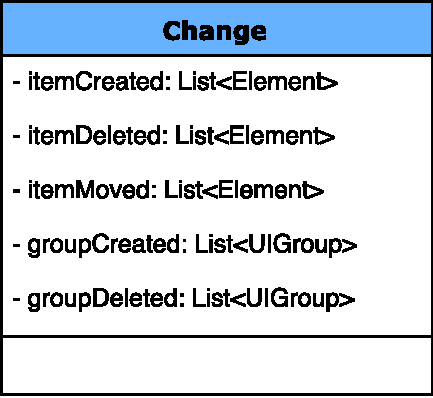
\includegraphics[width=0.5\textwidth]{figures/ClassDia_Change}
	\caption{Class Diagram for Change}
	\label{fig:ClassDia_Change}
\end{figure}

Actions performed by the user on both the views are tracked by the \texttt{Change} class. High-level view (Kitchen) allows three actions i.e., creation of a new item, deletion of an item and movement of an item. Whereas, low-level view (Grid) allows two actions i.e., creation of a new group and deletion of a group. Hence, \texttt{Change} class track all of these five actions separately. Figure~\ref{fig:ClassDia_Change} shows the class diagram of the \texttt{Change} class. It contains itemCreated, itemDeleted and ItemMoved as a list of \texttt{Element}s to capture creation, deletion and movement of an item respectively in high-level view. It also contains groupCreated and groupDeleted as a list of \texttt{UIGroup}s to capture creation and deletion of a group respectively in low-level view.

\subsubsection{View}\label{subsubsec:design_view}
The View handles the graphical user interface part of the application. Hence, it contains all the graphic elements and all other HTML elements of the application. View separates the design of the application from the logic of the application due to which the front end designer and the back end developer can work separately without thinking about the errors which could have showed up incase of an overlapping \cite{designpattern-headfirst} \cite{mvc-arch}. View controls how the data is being displayed, how the user interacts with it and provides ways for gathering the data from the users. 

In my case, the technologies that I am using for View are HTML, CSS and JavaScript and JQuery.

\paragraph{External Design}
For the visualization of the example \textit{Arranging a Kitchen} as explained in Section \ref{subsec:exampleforimplementation}, first task was to design the low-level and high-level views along with its functionalities.
\newline\newline Both the views represent a kitchen area and its certain behaviour. High-level view has more functionalities and flexibility in usage than the low-level view. As both the views are independent of each other and resonates a confined area in which certain task related to animation/graphics has to be performed, I chose \textit{Canvas} \cite{canvas} HTML element as a container for my views. \textit{Canvas} was the best fit for my views as it provides great support and application for creating animation and drawing graphics on web.

\begin{figure}
	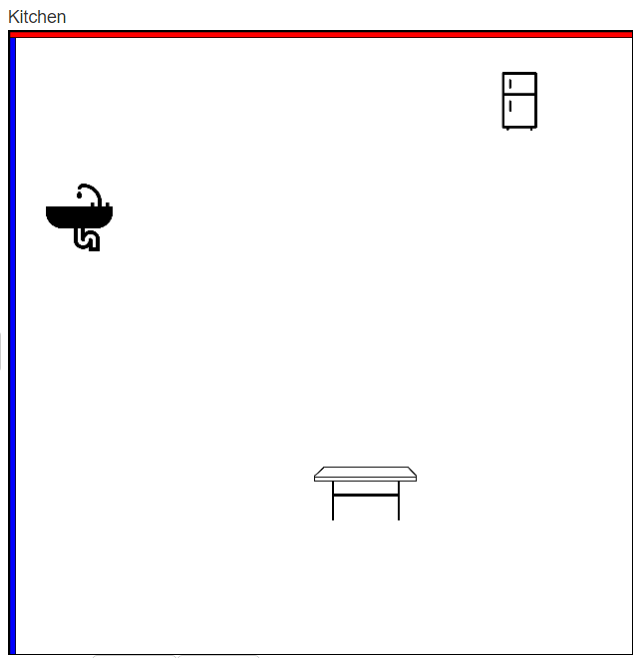
\includegraphics[width=0.7\textwidth]{figures/Highlevel_View}
	\caption{High Level View}
	\label{fig:HighLevel_View}
\end{figure}

For high-level view, I kept the \textit{Canvas} clean to represent an empty kitchen space where addition and manipulation of different objects such as, sink, table, fridge etc. can be done. Figure~\ref{fig:HighLevel_View} shows a sample of the high-level view (Kitchen View). To make the kitchen space more realistic, I have even added {\color{blue} water outlet} on western wall and {\color{red} electrical fittings} on northen wall so that the user can relate to it. For low-level view, I have filled the \textit{Canvas} with grids/blocks. The low-level view represents exact kitchen space as shown in high-level view but, divided into blocks. Also, the blocks restrict certain flexibility and functionality compared to high-level view. Figure~\ref{fig:LowLevel_View} shows a sample of the low-level view (Grid View).

\begin{figure}
	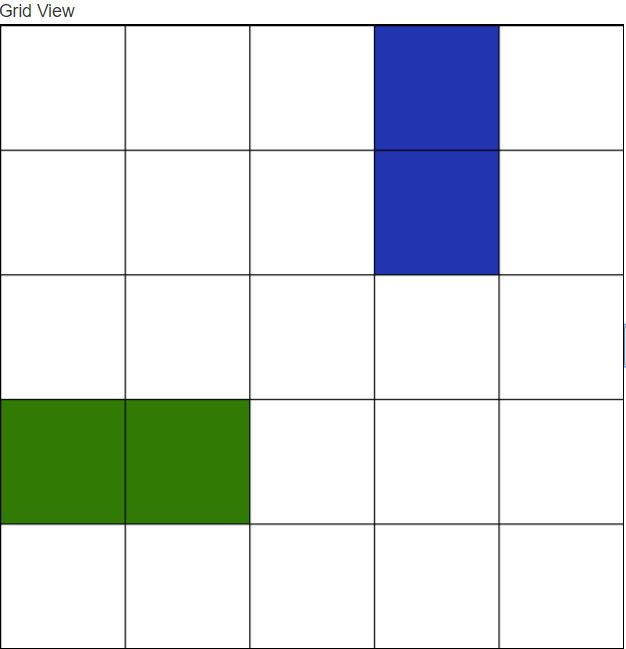
\includegraphics[width=0.7\textwidth]{figures/Lowlevel_View}
	\caption{Low Level View}
	\label{fig:LowLevel_View}
\end{figure}

Next step was to handle the user interactions in the process of performing various task on both the views. In web development, javascript is the most used language for handling the user intearctions and programming the behaviour of web pages \cite{javascript}. Hence, I have analyzed a few canvas libraries available in market e.g., Fabric.js \cite{fabricjs}, Processing.js \cite{processingjs}, Pixi.js \cite{pixijs}  by working on a few Proof of Concepts (PoC). The main idea was to check the feasibility and support for interactivity to perform different user defined tasks on the \textit{Canvas}. Finally, I chose Fabric.js as my javascript library for handling the user interactions because of below factors \cite{fabricjs}:
\begin{itemize}
	\item {It is good at displaying large number of objects on canvas.}
	\item {It handles object manipulation such as, moving, rotating, resizing for any kind of object.}
	\item {It has a great support for rendering and displaying object of any kind.}
\end{itemize}

\paragraph{Internal Design}
Second task in the process of visualization was defining the user actions with respect to both the views, capturing them, and displaying the views after transformation is done.

In high-level view, user can perform addition, removal and movement of the kitchen objects as it is done in everyone's house. A new object can be added and an already existing object can be moved or removed within the empty space available in the high-level view with the different mouse events. To make the example more realistic, I have used similar images of the kitchen objects as shown in figure~\ref{fig:HighLevel_View}. Every object is tracked on the basis of its position in the view and every change i.e., creation, deletion or movement of objects is captured inside a \textit{delta} by the high-level view and send it to the controller for further processing.

As low-level view offers less functionalities than high-level view, user can perform only addition and removal of the kitchen objects. Low-level view represents the kitchen space divided into blocks. Hence, each kitchen object is represented in the form of a group, combining any number of block(s) arranged in vertical or in horizontal direction filled with a unique color everytime a new object is added. For example, sink is represented by two horizontal blocks attached to one another and filled with {\color{blue} blue} color as shown in figure~\ref{fig:LowLevel_View}. As each object is identified with a group having an unique color, user can generate different colors by multiple mouse clicks on the non-occupied blocks while creating a new group. For deletion of a group, user can blur the color of an occupied block. Every group is tracked on the basis of the block's position that it is consist of along with its color and every change i.e., addition or removal is captured inside a \textit{delta} by the low-level view and send it to the controller for further processing.

After the changes are done on either view, to see the effect on the other, user can click on the synchronization button and both the views will be updated.
 
\subsubsection{Controller}\label{subsubsec:design_controller}
The Controller is mainly responsible for event/action handling and basically manages the relationship between a View and a Model \cite{mdd-webwithmvc}. These actions are triggered while a user is interacting with the application on a web browser. It accepts the user requests, interacts with
the Model, receives the response and generates the View.

In my case, I am using a thin Controller which is a Servlet along with a Controller helper consist of a java class.

\paragraph{Servlet \& Controller Helper}
Servlet is a technology which provides a component-based, platform-independent method for building web-based applications \cite{servlet}. Servlet is built on java platform to extend the capabilities of a web-server which makes it robust and scalable. It resides inside a web-server to generate dynamic content.

Servlet is capable of handling all kinds of client-server protocol but popularly and mostly used with the HTTP, the HyperText Transfer Protocol. A web container is essentially required to run a servlet. A web container is a component of the web server that interacts with the servlets and manages the lifecycle of servlets. In my case, I am using \textit{Apache Tomcat} as my web container. 

\begin{figure}
	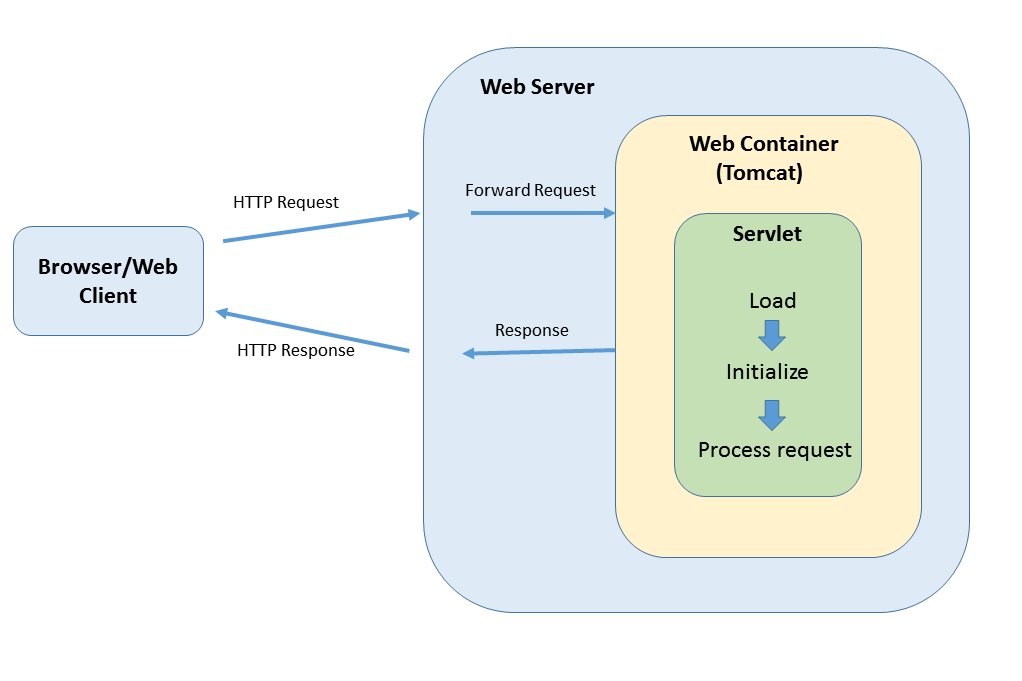
\includegraphics[width=1\textwidth]{figures/Server_Servlet}
	\caption{Servlet Lifecycle}
	\label{fig:Server_Servlet}
\end{figure}

Figure~\ref{fig:Server_Servlet} describes the complete lifecycle of a servlet w.r.t. a web server and a web container. The lifecycle steps are described as follows \cite{servlet}:
\begin{enumerate}
	\item {Web server receives the \texttt{HTTP request} from the client interacting through a browser.}
	\item {After accepting the request, web server forward the request to the web container i.e., tomcat.}
	\item {Web container sends the request to the \texttt{Servlet class}.}
	\item {If an instance of the servlet does not exist, the web container}\\\\
	loads the servlet class, then creates an instance of the servlet class and initializes the servlet instance by calling the \texttt{init} method.
	\item {After that, web container invokes the \texttt{service} methods (normally HTTP methods i.e., \texttt{get} , \texttt{post} , \texttt{put} , \texttt{delete}) of the servlet class by passing the request and response objects and the actual processing of the request is done and response is generated.}
	\item {Web container sends the response to the web server. Afterwards, web server creates the HTTP response and send it back to the client.}
\end{enumerate}

In my application, controller i.e., servlet is strongly coupled with a controller helper i.e., java class. Figure~\ref{fig:Controller_Workflow} describes the workflow of the Controller in my project. After invoking the service method of the servlet class, if an instance of the controller helper class does not exist, the servlet creates an instance of it and calls the appropiate method by passing the \texttt{UI Model} object. Inside the method of the controller helper, the conversion of the \texttt{UI Model} to the eMoflon specific models happens and data is sent to the \texttt{Model} for further processing. After processing, controller helper receives the response from the \texttt{Model} and conversion of the eMoflon specific models to the \texttt{UI Model} happens before sending the data to the servlet. 

\begin{figure}
	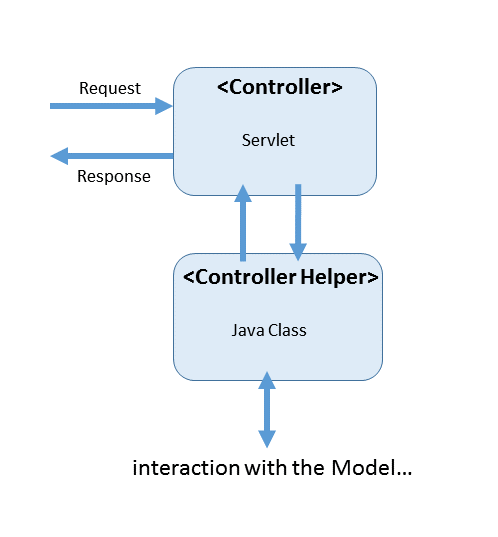
\includegraphics[width=1\textwidth]{figures/Controller_Workflow}
	\caption{Workflow within the Controller}
	\label{fig:Controller_Workflow}
\end{figure}

\subsection{Challenges}\label{subsec:designchallenges}
During the entire designing process as explained in previous sections of this chapter, I came across a few challenges. This section describes them in detail.

\paragraph{Architecture Design -- \textit{Avoiding circular dependency between projects}}
The first hurdle that I faced in the designing process was with application framework design. The challenge was correctly maintain the dependencies of projects without creating a circular dependency and strong coupling among each other. To overcome this challenge, basic concepts on design patterns and MVC architecture helped me in building the web architecture and maintaining the dependencies among the components in a correct way. 

\paragraph{UI Design -- \textit{Represent one workspace in two different views}}
UI design was the second big challenge that I faced during the designing process.

First problem was with the design, look, and feel of the high-level and low-level view. As per the requirement, both the views should represent the same workspace area but in different ways i.e, different action space, functionalities, and fexibility in interaction. So the challenge was to represent one workspace in two different views separated by functionalities and flexibility in use. Hence, I went through a few UI patterns \cite{designinterfaces} and scenarios based design principles \cite{scenariobasedui} for knowing the basics. Finally, I and my supervisor after a few discussions chose an empty canvas as shown in figure~\ref{fig:HighLevel_View} to represent high-level view and a canvas filled with blocks as shown in figure~\ref{fig:LowLevel_View} to represent low-level view.

\paragraph{UI Design -- \textit{Capturing different changes(delta) done in the views}}
Second problem was with conceptualizing the structure of \textit{delta} (refer Definition 3) by differentiating the functionalities e.g., changes done by user in the high-level and low-level view. So the challenge was to capturing different changes done in both the views but bundling them into one structure as the \textit{eMoflon} tool requires one input for all the changes done for transformation process. As mentionaed earlier, high-level and low-level view are different from each other based on their functionalities. For example, in high-level view three types of changes are allowed i.e., creation of a new item, deletion of an item, and movement of an item. Whereas, in low-level view two types of changes are allowed i.e., creation of a new group and deletion of a group. Hence, the structure of changes in both the views will be different as well. For separation of concerns, I decided to maintain five different variables for five different kinds of changes i.e., \texttt{createdItem}, \texttt{deletedItem}, \texttt{movedItem}, \texttt{createdGroup}, and \texttt{deletedGroup} but, bundled them into one single class \texttt{Change}. Also, a user can perform a series of changes even of the same type i.e., creating more than one item, deleting more than one item, creating more than one group etc., so I decided to keep every variable as a \texttt{List} item. Fig~\ref{fig:ClassDia_Change} shows the class diagram of the \texttt{Change} class and section \ref{subsubsec:design_model} explains the structure in deatil.

\subsection{Choices and Threats}\label{subsec:design_choicesthreats}
The implementation process and the final prototype was driven by many choices and threats. For example, 
\begin{itemize} 
	\item {selection of the bx tool and the most suitable example to implement has impact on deciding the usefullness of the demonstrator.}
	\item {seletion of the bx tool and the example to implement is more or less influenced by the ideas given by my supervisor.} 
	\item {my decisions on designing the application's framework for implementation are impacted by the existing availability and usability issues of the finalized bx-tool.}
	\item {During evaluation, I might not have got proper feedback from my friends \& colleagues due to my acquaintance and time constraints.}
\end{itemize}
